\documentclass[12pt]{article}
\usepackage[utf8]{inputenc}
\newcommand\preamble{
    \usepackage[italian]{babel}
    \usepackage{geometry}
    \usepackage{amsmath}
    \usepackage{amssymb}
    \usepackage{graphicx}
    \usepackage{ulem}
    \usepackage[dvipsnames]{xcolor}

    \geometry{margin=2cm}
    \let\olditemize\itemize
    \renewcommand\itemize{\olditemize\setlength\itemsep{0em}}
    \graphicspath{{../Immagini/}}

    \author{Lorenzo Vaccarecci}
}
\preamble

\title{Gestione delle Strutture Ausiliarie di Accesso (Indici)}
\date{15 Marzo 2024}

\begin{document}
\maketitle
\section{Esempio}
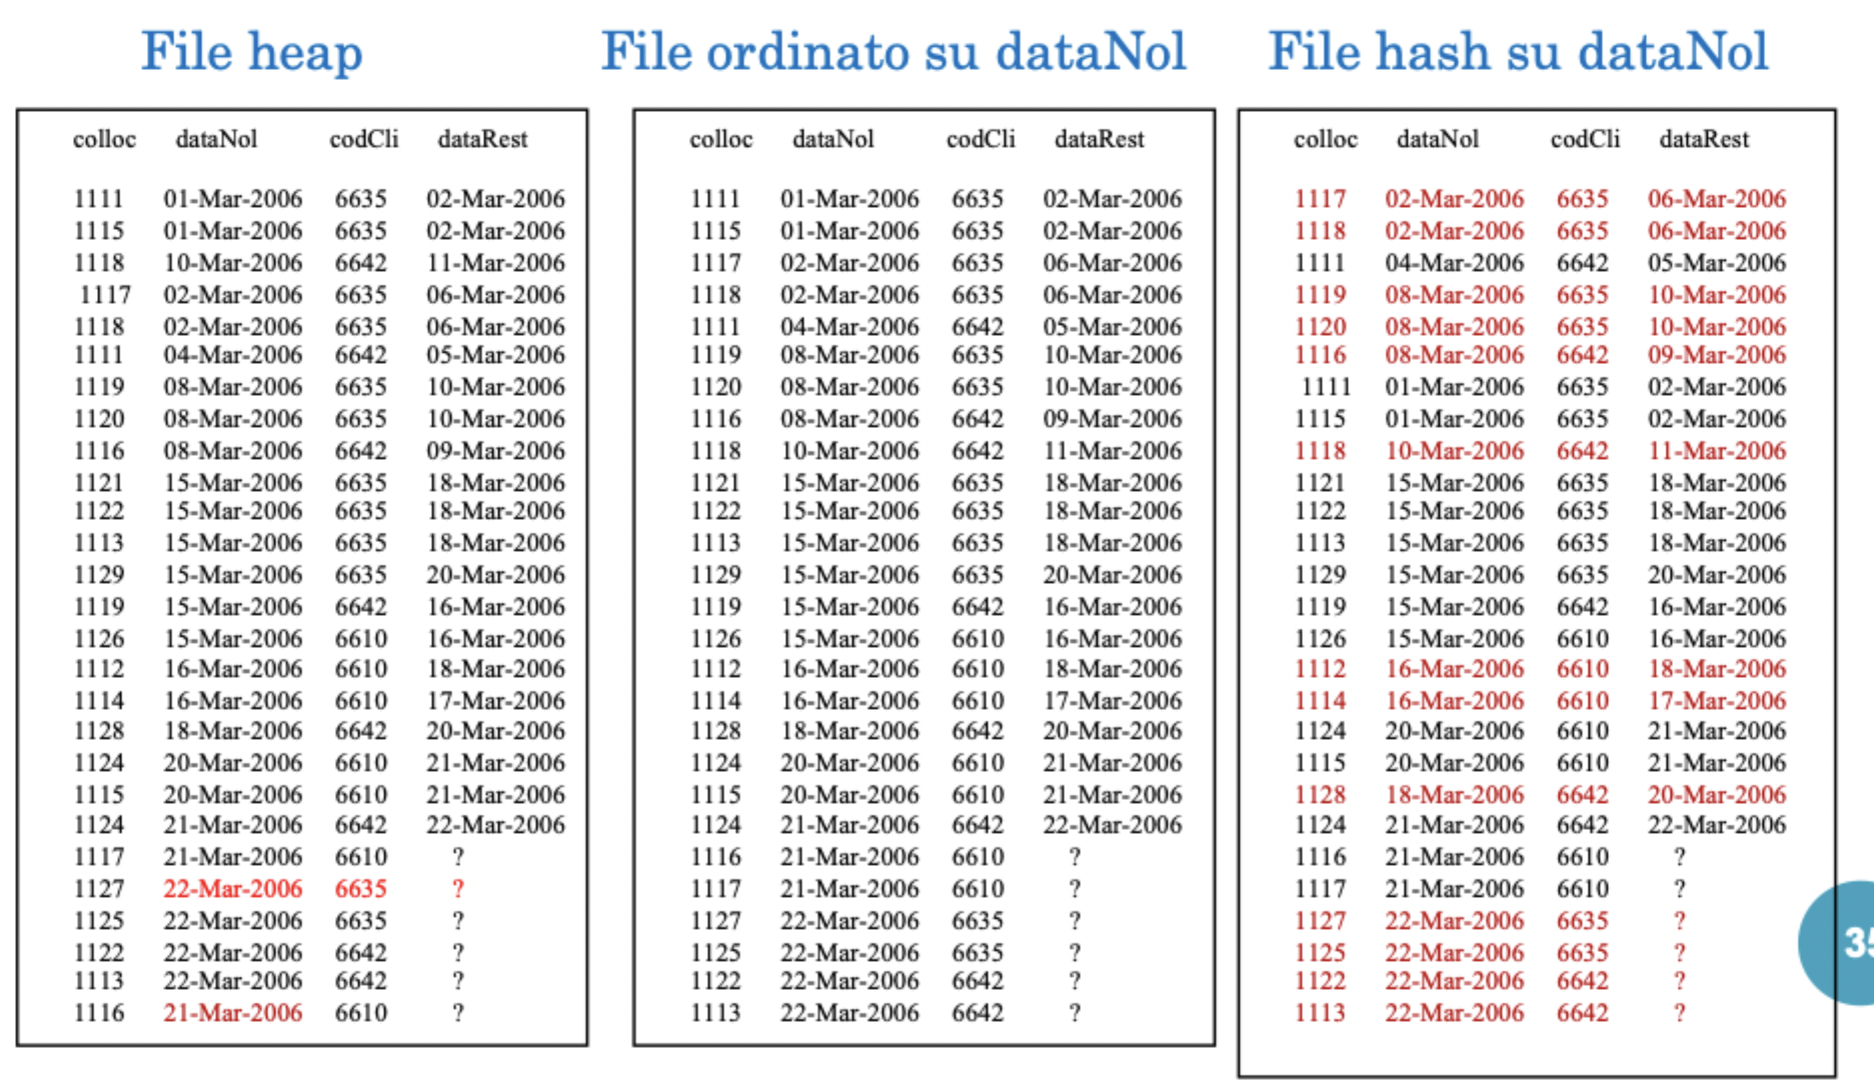
\includegraphics[width=\textwidth]{recordfile.png}
Supponiamo di voler recuperare tutti i noleggi effettuati in una certa data nel file ordinato su \textit{dataNol}. 
\begin{itemize}
    \item A \textcolor{Cyan}{ livello logico}: descrizione richiesta in modo dichiarativo
    \item A \textcolor{Cyan}{livello fisico}: algoritmo che implementa a livello fisico la richiesta, ad esempio:
    \begin{itemize}
        \item apri il file che contiene i record
        \item doppio while per il file e per il blocco di dati nel file dove controlliamo se la data è quella che ci interessa
    \end{itemize}
\end{itemize}
Ho dovuto leggere tutti i blocchi di dati prima della data per trovare i record che mi interessano. \textit{Bene ma non benissimo: basti pensare a un file con migliaia di record.}\newpage
Supponiamo ora di voler recuperare tutti i noleggi effettuati con un certo colloc nel file ordinato su \textit{dataNol}.
\begin{itemize}
    \item A \textcolor{Cyan}{ livello logico}: descrizione richiesta in modo dichiarativo
    \item A \textcolor{Cyan}{livello fisico}: algoritmo che implementa a livello fisico la richiesta, ad esempio:
    \begin{itemize}
        \item apri il file che contiene i record
        \item doppio while per il file e per il blocco di dati nel file dove controlliamo se colloc è quello che ci interessa
    \end{itemize}
\end{itemize}
Ho dovuto leggere tutti i blocchi di dati per trovare i record che mi interessano. \textit{Non efficiente, devo leggere tutto il file.}
\section{Perchè gli indici}
Sono delle strutture ausiliare create dal sistema per velocizzare l'accesso ai dati. Gli indici riferiti a una chiave ordinata è detto \textbf{clusterizzato}, altrimenti \textbf{non clusterizzato}.
\begin{center}
    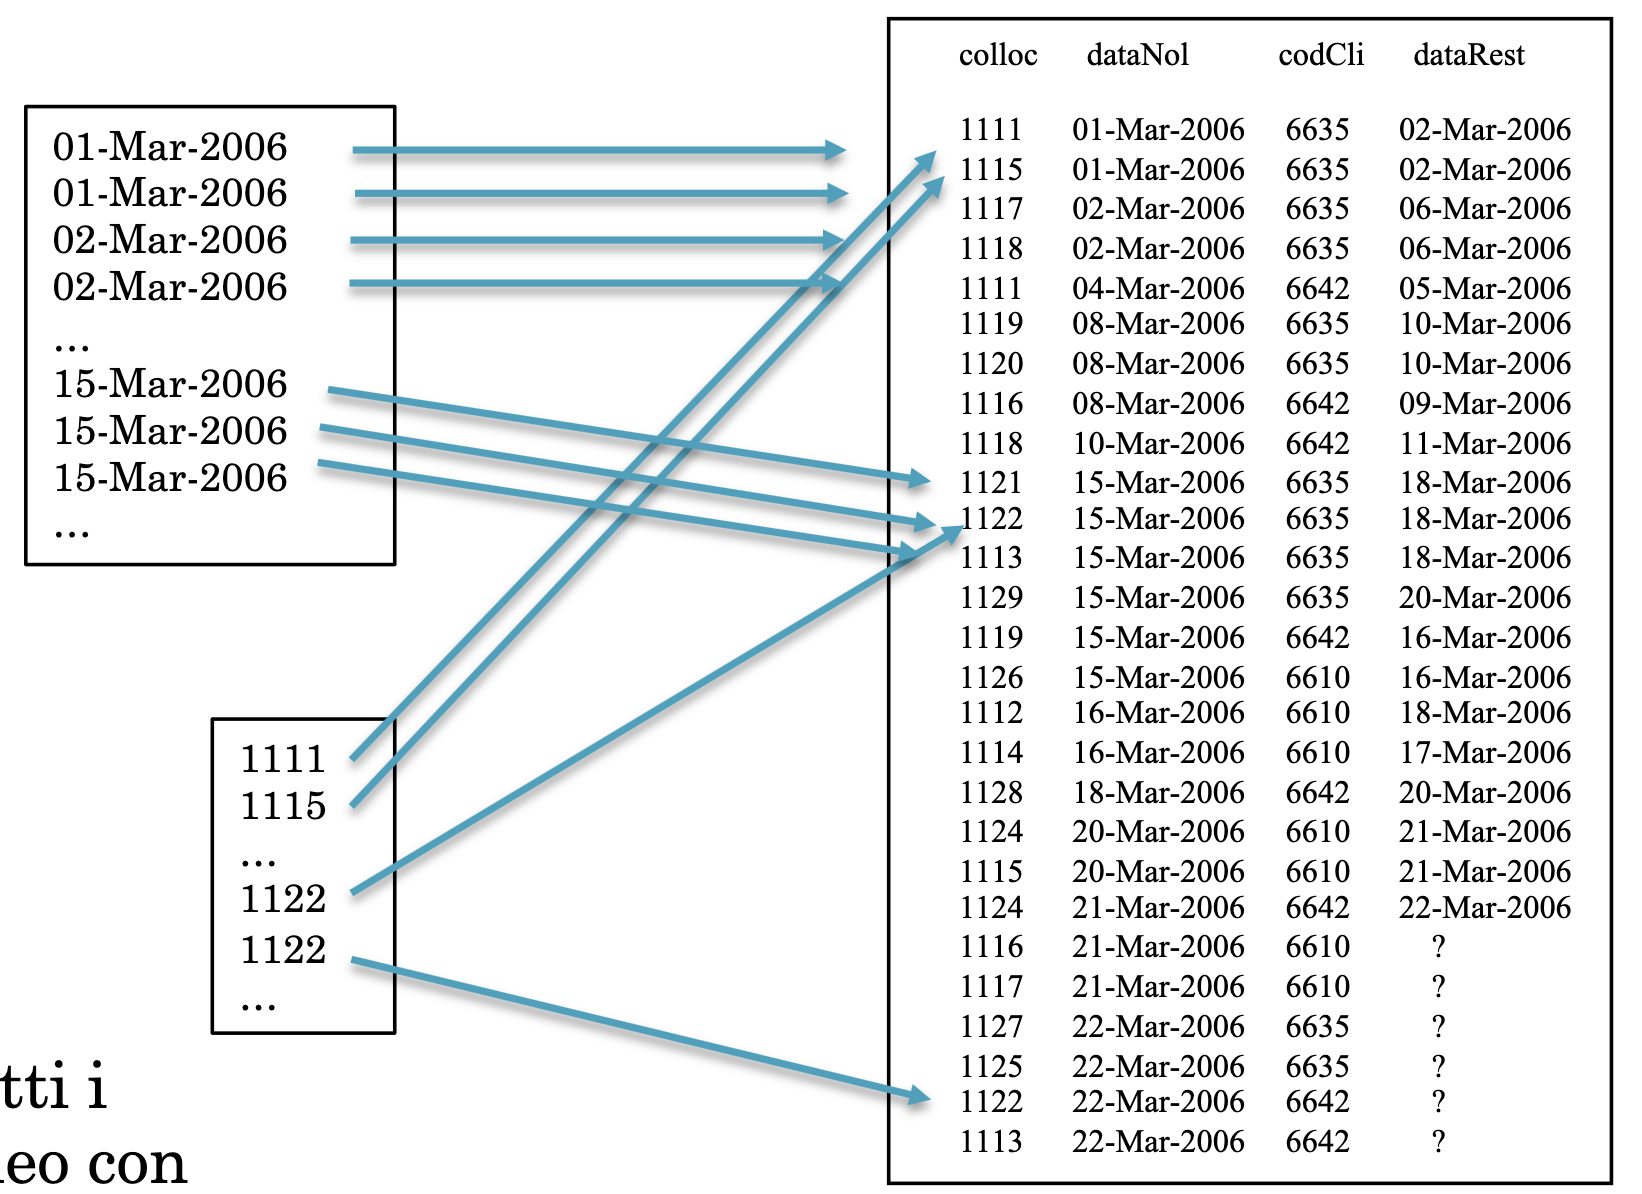
\includegraphics[width=\textwidth]{indici.png}
\end{center}
Un indice su una relazione $R$ è un insieme di coppie del tipo $\{(k_{i}, r_{i}),\dots,(k_{n}, r_{n})\}$ dove $k$ è un valore $x$ un attributo (o un insieme di attributi) chiamato chiave di ricerca e $r$ è un puntatore al file dei dati.
\section{Accesso con indice}
\begin{center}
    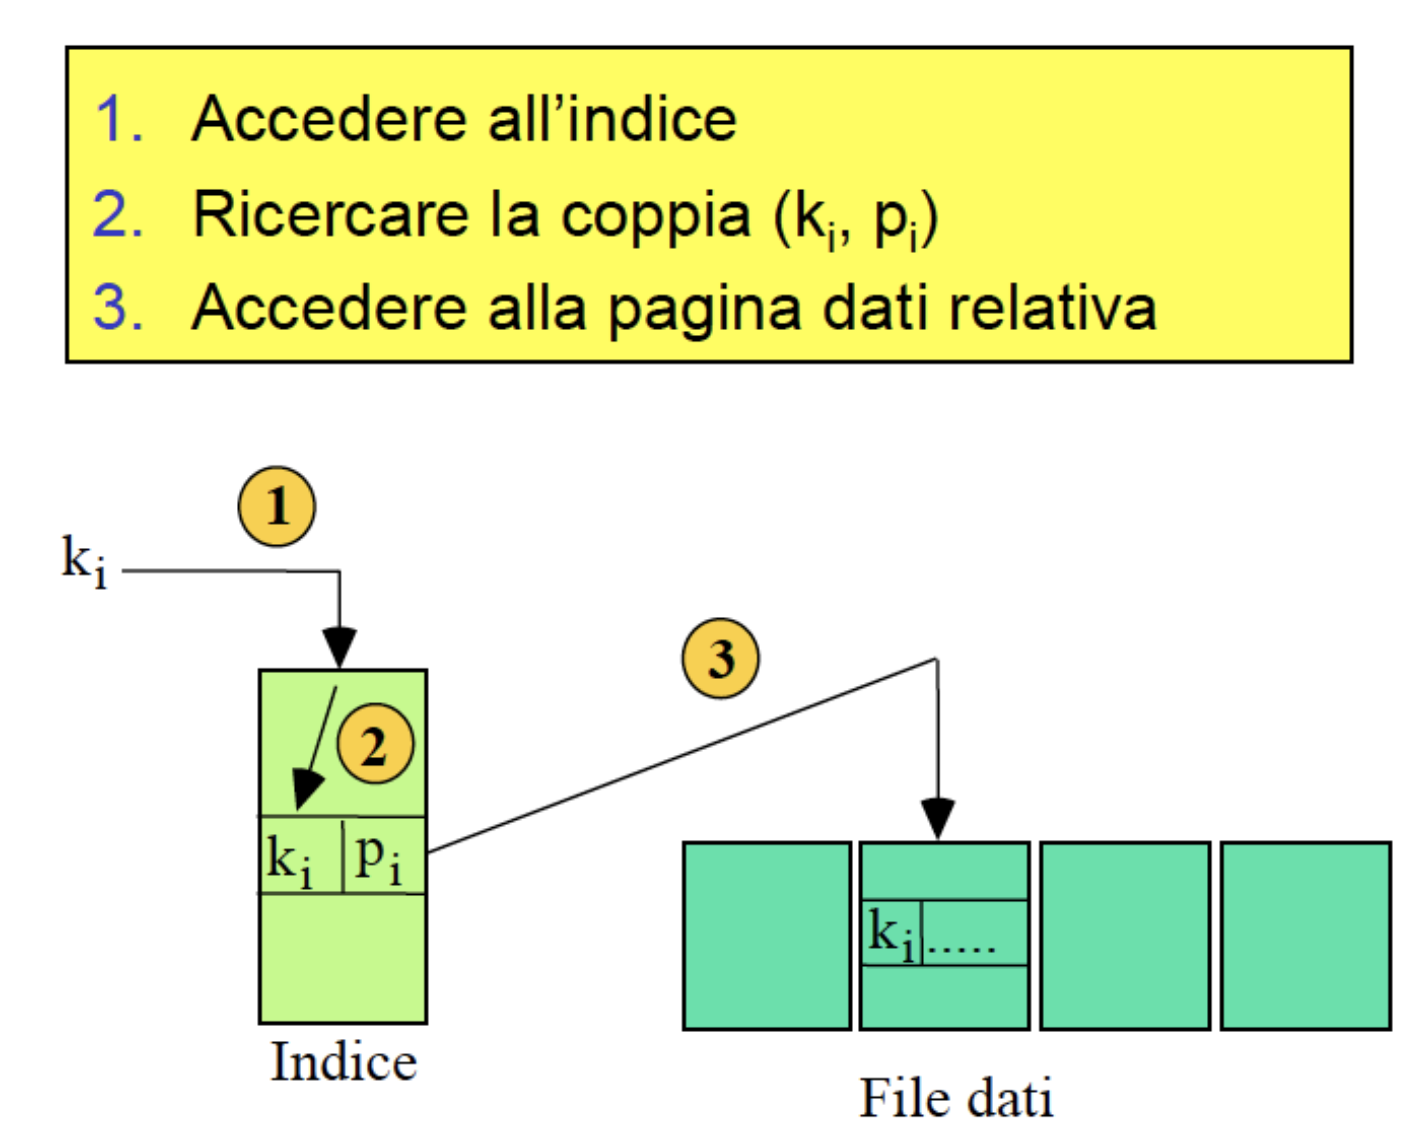
\includegraphics[scale=0.5]{accessoindici.png}
\end{center}
\section{Indici e Aggiornamenti}
Gli indici rendono efficiente l'esecuzione delle interrogazioni ma rendono più complessi gli aggiornamenti (ogni volta che si aggiorna il file dei dati bisogna aggiornare anche l'indice).
\begin{center}
    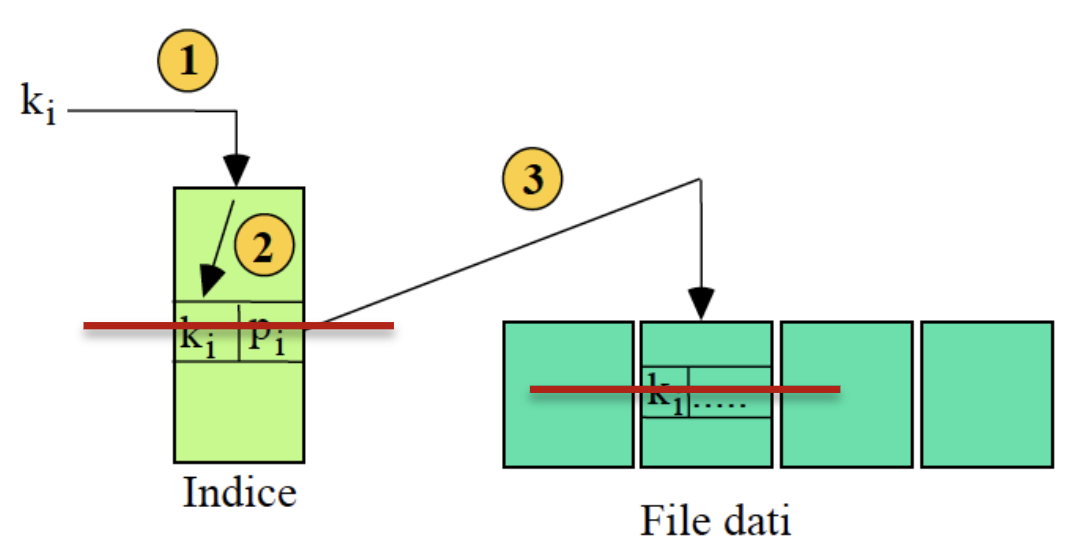
\includegraphics[width=\textwidth]{aggiornamentoindici.png}
\end{center}
\section{Indici primari e secondari}
\begin{description}
    \item[Primari]: se la chiave di ricerca soddisfa il vincolo di unicità
    \item[Secondari]: se la chiave di ricerca non soddisfa il vincolo di unicità, per evitare di replicare inutilmente lo stesso valore si raggruppano le chiavi associando una lista di puntatori.
\end{description}
\begin{center}
    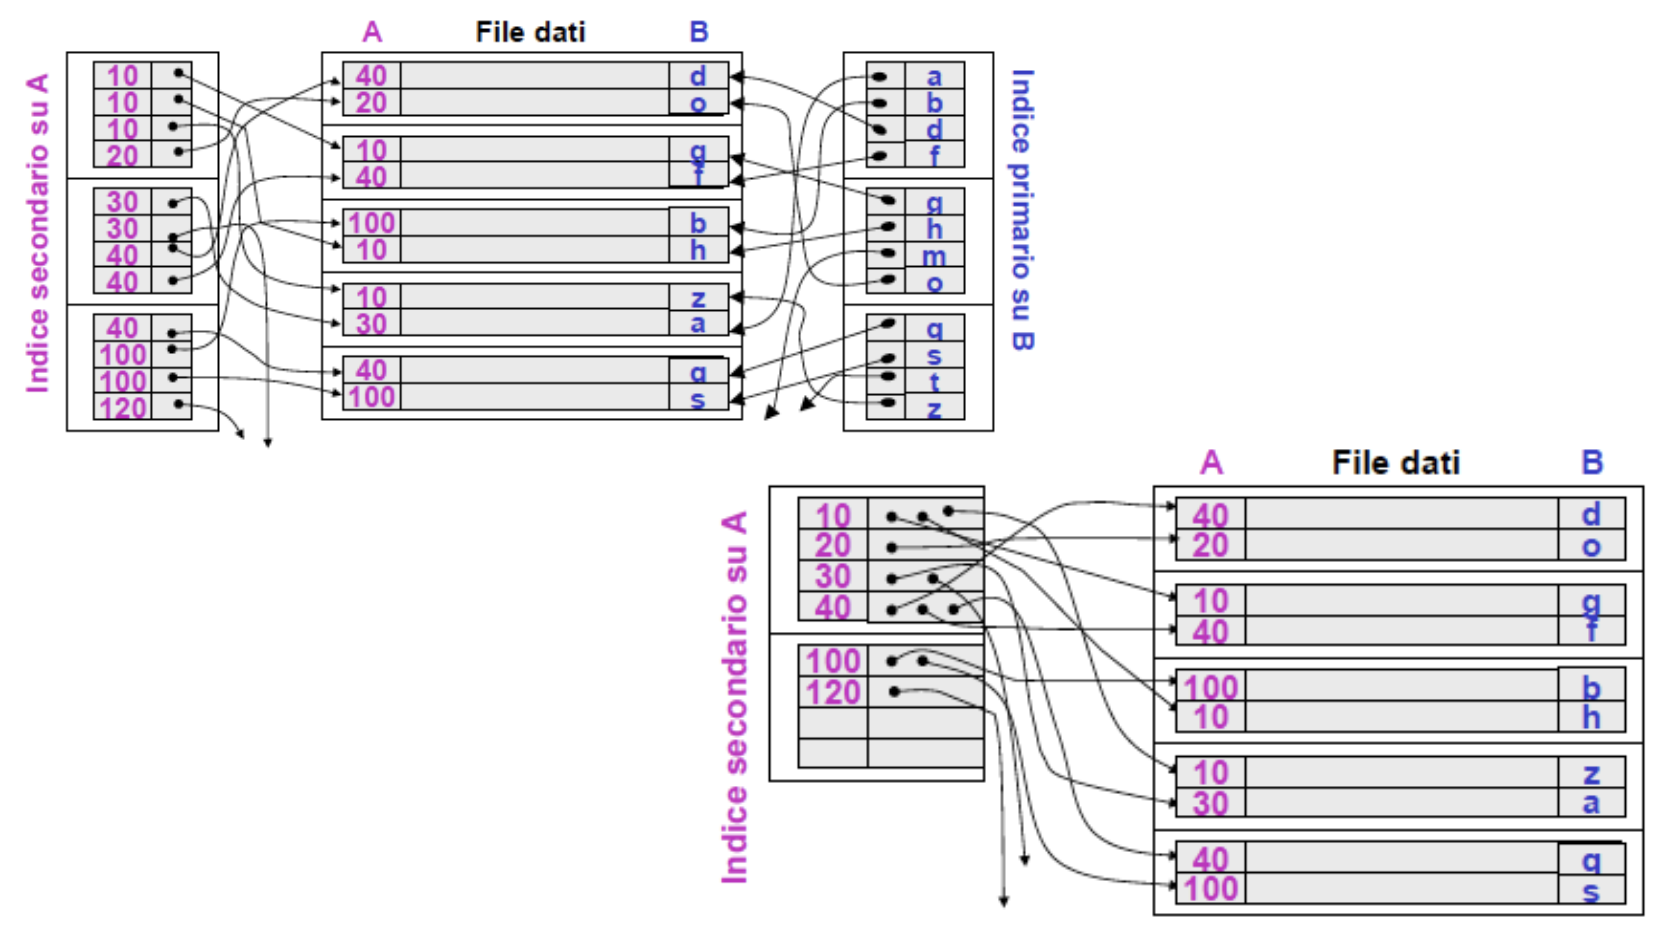
\includegraphics[width=\textwidth]{primarisecondari.png}
\end{center}
\section{Tipi di indici}
\begin{description}
    \item[Ordinati]: o indici ad albero, le coppie $(k_{i},r_{i})$ vengono salvate in un file ordinate rispetto ai valori della chiave $k_{i}$
    \item[Hash]: le coppie non vengono memorizzate su un file ma "calcolate" attraverso l'uso di una funzione hash $h(k_{i})=r_{i}$
\end{description}
\end{document}